\documentclass{letask}

\begin{document}
\begin{titlepage}
\center % Center everything on the page
 
%----------------------------------------------------------------------------------------
%	HEADING SECTIONS
%----------------------------------------------------------------------------------------

\textsc{\LARGE Московский\\[-0.2cm]Физико-Технический Институт\\[0.1cm]\large (государственный университет)}\\[1.5cm] % Name of your university/college
\textsc{\Large Кафедра общей физики}\\[0.1cm] % Major heading such as course name
\textsc{\large Лабораторная работа \textnumero  4.4.1}\\[0.5cm] % Minor heading such as course title

%----------------------------------------------------------------------------------------
%	TITLE SECTION
%----------------------------------------------------------------------------------------

\HRule
\\[0.4cm]
{ \huge \bfseries Амплитудная\\[0.2cm]
дифракционная решетка}
\\[0.6cm] % Title of your document
\HRule
\\[1.5cm]


 
%----------------------------------------------------------------------------------------
%	AUTHOR SECTION
%----------------------------------------------------------------------------------------

\begin{minipage}{0.4\textwidth}
	\begin{flushleft} \large
		\textsf{Студент}
		
		Ришат \textsc{Исхаков} \\[-0.15cm]
		513 группа
	\end{flushleft}
\end{minipage}
~
\begin{minipage}{0.4\textwidth}
	\begin{flushright} \large
		\textsf{Преподаватель}
		
		Александр Александрович \\[-0.15cm]
		\textsc{Казимиров} % Supervisor's Name
	\end{flushright}
\end{minipage}

\begin{bottompar}
	\begin{center}
		
\includegraphics[width = 80 mm]{logo.jpg}
	\end{center}
	{\large \today}

\end{bottompar}
\vfill % Fill the rest of the page with whitespace

\end{titlepage}

\textbf{Цель работы:} исследовать явления дифракции Френеля и Фраунгофера на щели, изучить влияние дифракции на разрешающую способность оптических инструментов.

\textbf{В работе используются:} оптическая скамья, ртутная лампа, монохроматор, щели с регулируемой шириной, рамка с вертикальной нитью, двойная щель, микроскоп на поперечных салазках с микрометрическим винтом, зрительная труба.

\section{Дифракция Френеля на щели}

Схема установки для наблюдения дифракции Френеля представлена на рис. 1. Световые лучи освещают щель S2 и испытывают на ней дифракцию. Дифракционная картина рассматривается с помощью микроскопа М, сфокусированного на некоторую плоскость наблюдения П.

\begin{figure}[H]
\centering
	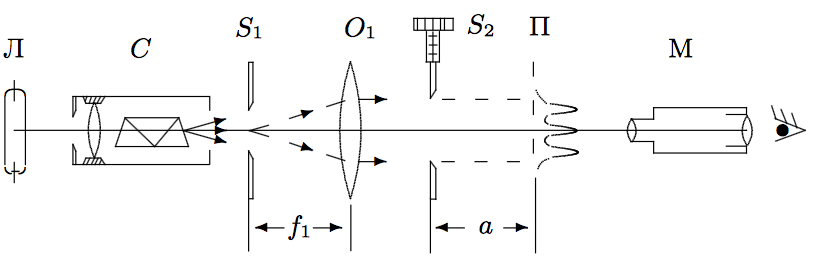
\includegraphics[width = \lw]{img1}
	\caption{Схема установки для наблюдения дифракции Френеля}
	\label{fig:scheme}
\end{figure}


Щель S2 освещается параллельным пучком монохроматического света с помощью коллиматора, образованного объективом O1 и щелью S1, находящейся в его фокусе. На щель S1 сфокусировано изображение спектральной линии, выделенной из спектра ртутной лампы Л при помощи простого монохроматора C, в котором используется призма прямого зрения. 

Распределение интенсивности света в плоскости наблюдения П проще всего рассчитывать с помощью зон Френеля (для щели их иногда называют зонами Шустера). При освещении щели S2 параллельным пучком лучей (плоская волна) зоны Френеля представляют собой полоски, параллельные краям щели (рис. 2). Результирующая амплитуда в точке наблюдения определяется суперпозицией колебаний от тех зон Френеля, которые не перекрыты створками щели. Графическое определение результирующей амплитуды производится с помощью векторной диаграммы — спирали Корню. Суммарная ширина $m$ зон Френеля $z_m$ определяется соотношением: 
\[ z_m = \sqrt{am\lambda}, \]

где a~--~расстояние от щели до плоскости наблюдения (рис. \ref{fig:scheme}), а $\lambda$~--~длина волны.

\textbf{Измерим значение расстояний при изменении количества темных полос:}

\begin{table}[H]
\centering
\caption{Зависимость расстояния от количества полос}
\begin{tabular}{|c|c|c|c|c|c|}
\hline
$n$          & 5      & 4      & 3      & 2      & 1      \\ \hline
$z$          & 0.8    & 1.1    & 1.4    & 1.8    & 2.6    \\ \hline
$2\xi$       & 323.81 & 346.62 & 349.75 & 343.45 & 337.03 \\ \hline
$\delta x$   & 0.05   & 0.05   & 0.05   & 0.05   & 0.1    \\ \hline
$\epsilon x$ & 0.06   & 0.05   & 0.04   & 0.03   & 0.04   \\ \hline
$\delta \xi$  & 20.24  & 15.76  & 12.49  & 9.54   & 12.96  \\ \hline
\end{tabular}
\end{table}

Построим график зависимости $2 \xi_n (n) $:

\begin{figure}[H]
\centering
  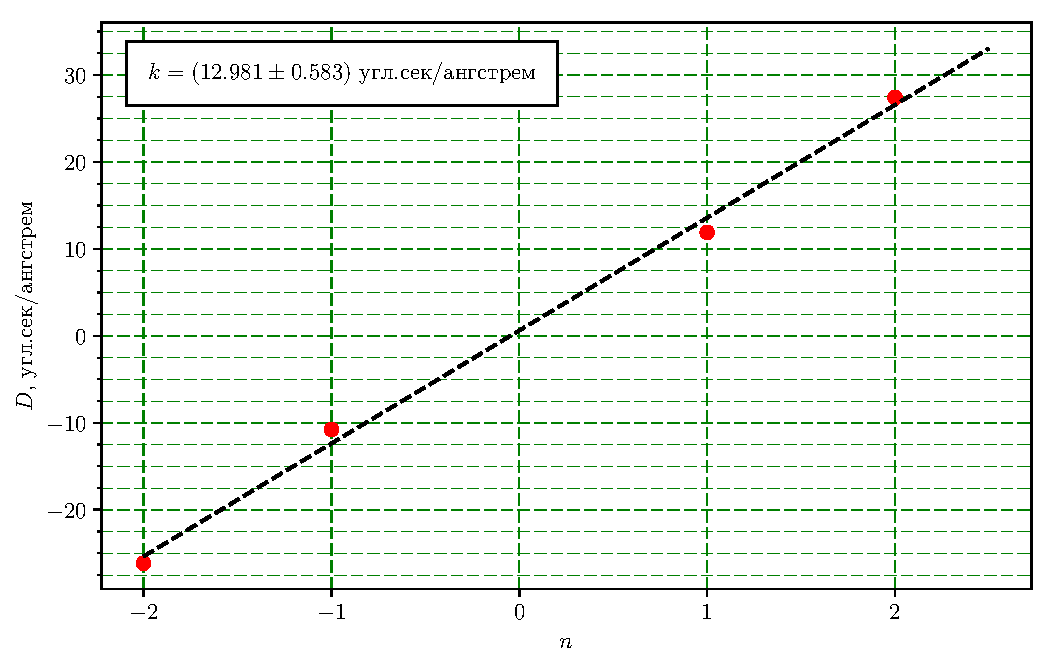
\includegraphics[width = 0.9 \lw]{graph1}
  \caption{График зависимости $2 \xi_n (n)$}
\end{figure}

\section{Дифракция Фраунгофера на щели}

Картина дифракции резко упрощается, когда ширина щели становится значительно меньше ширины первой зоны Френеля. 

Это условие всегда выполняется при достаточно большом расстоянии a от щели до плоскости наблюдения. Дифракционную картину, наблюдаемую в этом случае, принято называть дифракцией Фраунгофера. Исследование такой дифракционной картины заметно облегчается, потому что упрощаются фазовые соотношения.

Дифракцию Френеля и Фраунгофера можно наблюдать на одной и той же установке (рис.~1). Однако при обычных размерах установки дифракция Фраунгофера возникает только при очень узких щелях. Например, при $a \approx 20-40~\cm$ и $\lambda \approx 5 \cdot 10^{-5}~\cm$ получаем $D \ll 0.3~\mm$. Поскольку работать с такими тонкими щелями неудобно, для наблюдения дифракции Фраунгофера к схеме, изображённой на рис. 1 добавляется объектив $O_2$ (рис.~\ref{img:fraung}).

\begin{figure}[H]
\centering
  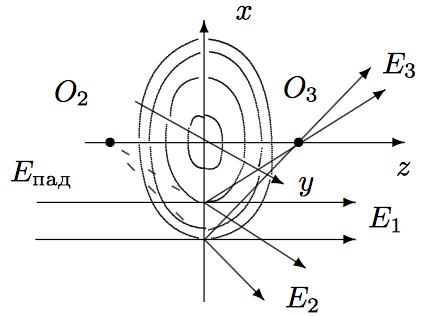
\includegraphics[width = 0.9 \lw]{img2}
  \caption{Схема установки для наблюдения дифракции Фраунгофера на щели}
  \label{img:fraung}
\end{figure}

Дифракционная картина наблюдается здесь в фокальной плоскости объектива $O_2$.

\textbf{Начальные данные:}
\[f_1 = 11~\cm\]
\[f_2 = 12.5~\cm\]

\begin{table}[H]
\centering
\caption{Координаты дифракционных минимумов}
\begin{tabular}{|c|c|c|c|c|c|c|c|c|c|}
\hline
$m$        & -4   & -3   & -2   & -1   & 0   & 1    & 2    & 3   & 4    \\ \hline
$x_m, \mm$ & 0.62 & 0.85 & 1.03 & 1.25 & 1.5 & 1.68 & 1.88 & 2.1 & 2.32 \\ \hline
\end{tabular}
\end{table}

Построим график зависимости $x_m(m)$:

\begin{figure}[H]
  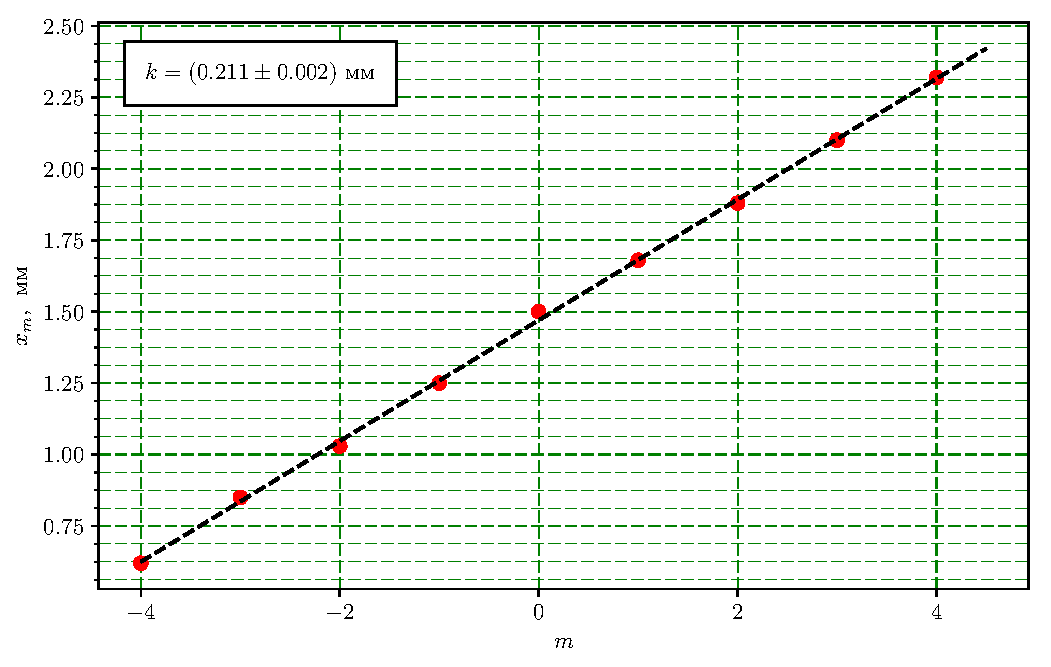
\includegraphics[width = 0.9 \lw]{graph2}
  \caption{Зависимость $x_m(m)$}
\end{figure}

Рассчитаем ширину щели $b$:
\[b = \dfrac{f_2 \lambda}{k} = 0.32~\mm \]

\section{Дифракция Фраунгофера на двух щелях}

\begin{figure}[H]
  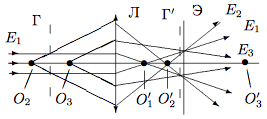
\includegraphics[width = 0.9 \lw]{img3}
  \caption{Схема установки для наблюдения дифракции Фраунгофера на двух щелях}
  \label{img:fraung_2}
\end{figure}


Для наблюдения дифракции Фраунгофера на двух щелях в установке (рис. \ref{img:fraung}) следует заменить щель $S_2$ экраном Э с двумя щелями (рис. \ref{img:fraung_2}). При этом для оценки влияния ширины входной щели на чёткость ди- фракционной картины вместо входной щели $S_1$ следует поставить щель с микрометрическим винтом. Два дифракционных изображения входной щели, одно из которых образовано лучами, прошедшими через левую, а другое — через правую щели, накладываются друг на друга.

Если входная щель достаточно узка, то дифракционная картина в плоскости П (рис. \ref{img:fraung}) подобна той, что получалась при дифракции на одной щели (рис. \ref{img:fraung_2}), однако теперь вся картина испещрена рядом дополнительных узких полос. Наличие этих полос объясняется суперпозицией световых волн, приходящих в плоскость наблюдения через разные щели экрана Э.

 \begin{enumerate}
  \item Определим координаты $x_1, x_2$ самых удаленных друг от друга темных полос внутри первого максимума, а также координату центра максимума:
\[x_1 = 
  \item 
\end{enumerate}


\section{Установка и параметры измерения}

\section{Вывод}
\end{document}
